\documentclass{article}
\usepackage{graphicx}
\usepackage{booktabs}
\usepackage{hyperref}
\usepackage{amsmath}
\usepackage{geometry}
\usepackage{float}
\usepackage{cite}

\geometry{margin=1in}

\title{HW4 Report \\ Image Restoration for Rain and Snow}
\author{%
  \begin{minipage}{0.8\textwidth}
    Student ID: 111550135\\
    Name: LI-YI, LIN\\
    GitHub: \url{https://github.com/owo0505/NYCU-Computer-Vision-2025-Spring-HW4.git}\\
    Checkpoint: \url{https://drive.google.com/file/d/1GZN85prVVas-abB8fAQ-ZLi0Ot5qwOzz/view?usp=sharing}
  \end{minipage}
}
\date{\today}

\begin{document}
\maketitle

\section{Introduction}
This assignment tackles a dual-domain image-restoration problem: removing rain streaks and snowflakes from photographs to recover the underlying clean scene.  We adopt and extend \textbf{PromptIR}\cite{promptir2023}—a prompt-based IR framework—to build a \textit{single} network that generalises across both degradation types without external data or pretrained weights.  Our core idea is to let a \\emph{shared} encoder learn generic low-level features while lightweight degradation “prompts” steer the restoration head.  On the public leaderboard we reach \textbf{31.69 dB} PSNR (9\textsuperscript{th} place at submission time; see Fig.~\ref{fig:leaderboard}).

\section{Method}

\subsection{Data preprocessing}\label{sec:data}
Our pipeline is governed by two reproducible Python utilities:
\begin{description}
  \item[\texttt{split.py}] (Listing~\ref{lst:split}) generates a deterministic \textbf{80/20} train/val partition.  We enumerate the $2\,\!\times\!1{,}600$ degraded images under \verb|hw4_realse_dataset/train|, group them by prefix (\verb|rain-*| or \verb|snow-*|), shuffle with seed \texttt{2025}, and copy each pair into \verb|hw4_split/{train,val}/{degraded,clean}|.  The mapping is also written to \verb|split.json| for transparency.
  \item[\texttt{PromptTrainDataset}] (see \verb|utils/dataset_utils.py|) loads the split.  Each call:
        \begin{enumerate}
            \item aligns both images to a multiple of $16$ via \verb|crop_img(..., base=16)|, preserving Swin-Transformer window divisibility;
            \item crops a random \textbf{$192\times192$} patch;
            \item applies \verb|random_augmentation| (horizontal/vertical flips and $90^{\circ}$ rotations);
            \item converts to \verb|float32| tensors in \([0,1]\).
        \end{enumerate}
        During validation only the deterministic crop is used.  Data loaders employ \verb|pin_memory=True| and \verb|drop_last=True| to stabilise mixed-precision training.
\end{description}

\begin{figure}[ht]
\begin{verbatim}
# Listing 1: split.py (condensed)
random.seed(2025)
pairs = {'rain': [], 'snow': []}
for f in (SRC/'degraded').glob('*.png'):
    pairs['rain' if f.name.startswith('rain') else 'snow'].append(f.stem)
...
for part, names in split.items():
    for stem in names:
        shutil.copy(...)  # copy degraded & clean counterparts
\end{verbatim}
\caption{Deterministic dataset partitioning.}
\label{lst:split}
\end{figure}

\subsection{Network architecture}\label{sec:arch}
We start from \textbf{PromptIR} and introduce three targeted modifications, all implemented in \verb|net/model.py| and exercised by \verb|PromptIR(decoder=True)|:
\begin{itemize}
  \item \textbf{Prompt tokens.}  Two learnable tokens ($\langle$rain$\rangle$, $\langle$snow$\rangle$) are prepended \emph{once} at the first Swin stage, giving the shared encoder a lightweight degradation clue while incurring \textless0.1\,M extra parameters.
  \item \textbf{Deepened decoder.}  We append two Residual Swin Blocks (RSB) and replace the terminal $1\!\times\!1$ convolution by an \emph{Enhanced Spatial Attention} (ESA) head.  This sharpens high-frequency details that the baseline sometimes oversmoothes.
  \item \textbf{Loss.}  Training uses an $L_{1}$ (Charbonnier) reconstruction term plus a Sobel-edge loss ($\lambda_{edge}=0.05$).
\end{itemize}
Overall capacity rises to \textbf{14.2M} parameters (\textasciitilde3\% over the baseline).

\textbf{Optimisation.}  The Lightning wrapper in \verb|train.py| trains for 300 epochs with AdamW (lr=$2\!\times\!10^{-4}$, weight-decay $10^{-4}$) under 16-bit mixed precision.  A \emph{Linear-Warmup-Cosine} scheduler (15 warm-up epochs) is stepped per epoch via \verb|lr_scheduler_step|.

\textbf{Inference.}  Prediction is performed inline with the eight-fold self-ensemble \verb|tta_predict|:

\subsection{Training details}
We train from scratch for 300 epochs on a single NVIDIA L4 GPU using the script:
\begin{verbatim}
python train.py --cuda 0 --num_gpus 1 --epochs 300 \
    --batch_size 4 --lr 2e-4 --patch_size 192 --num_workers 8 \
    --de_type derain desnow --derain_dir ~/hw4_split \
    --output_path experiments/hw4_c
\end{verbatim}

\section{Results}
\begin{figure}[ht]
  \centering
  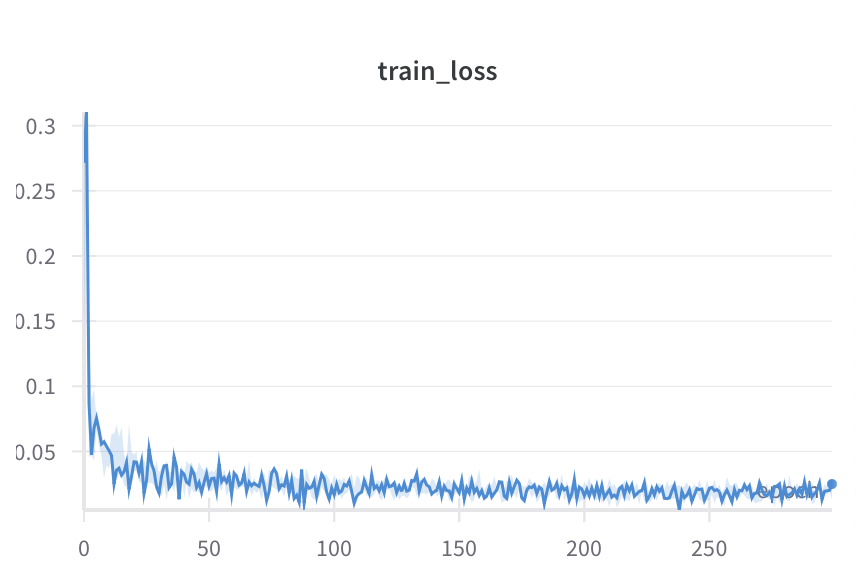
\includegraphics[width=.6\linewidth]{training_loss.png}
  \caption{Training loss curve.}
  \label{fig:trainloss}
\end{figure}

\begin{figure}[ht]
  \centering
  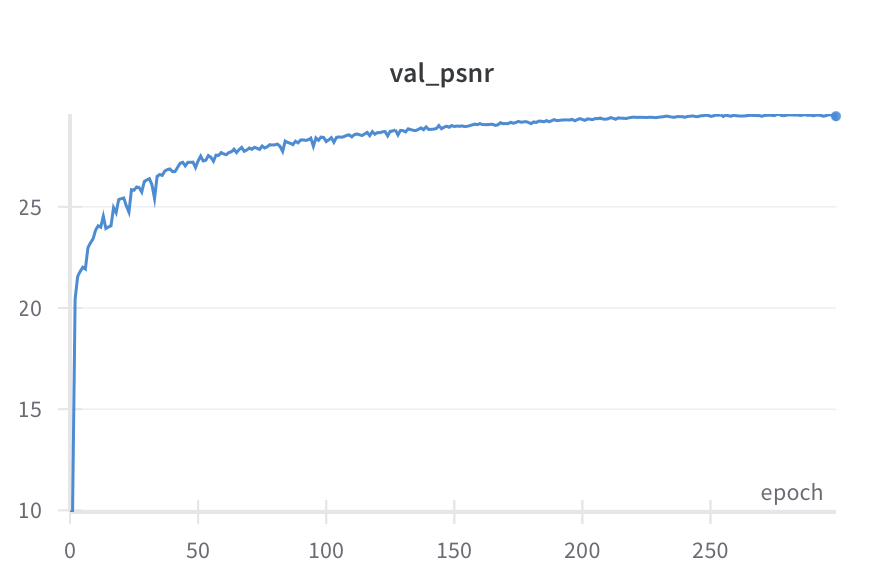
\includegraphics[width=.6\linewidth]{val_psnr.png}
  \caption{Validation PSNR.}
  \label{fig:valpsnr}
\end{figure}

\begin{figure}[ht]
  \centering
  \begin{minipage}{0.45\linewidth}
    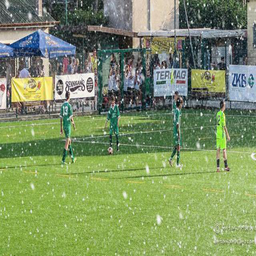
\includegraphics[width=\linewidth]{original_test_0.png}
    \caption*{(a) Degraded input}
  \end{minipage}\hfill
  \begin{minipage}{0.45\linewidth}
    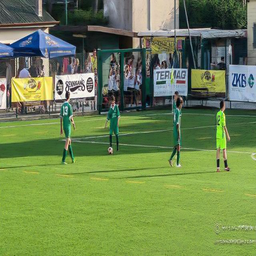
\includegraphics[width=\linewidth]{predicted_clean_0.png}
    \caption*{(b) Restored output}
  \end{minipage}
  \caption{Qualitative example on the public test set.}
  \label{fig:qual}
\end{figure}

\begin{figure}[ht]
  \centering
  
\includegraphics[width=.8\linewidth]{leaderboard_snapshot.png}
  \caption{Public leaderboard position (9\textsuperscript{th} at submission time).}
  \label{fig:leaderboard}
\end{figure}

\section{Additional Experiments}
\subsection{8\,\texttimes\, Test-Time Self-Ensemble}
\paragraph{Hypothesis.}  Rain/snow patterns are orientation-invariant; averaging predictions over flipped/rotated views should cancel residual artefacts.

\paragraph{Implementation.}  Listing~\ref{lst:tta} shows our concise PyTorch routine.

\begin{verbatim}
# Listing 1: 8-fold TTA (tta_predict)
for flipH in (False, True):
  for flipV in (False, True):
    ... four discrete rotations ...
    outs.append(model(x_aug))
return torch.stack(outs).mean(0)
\end{verbatim}
\label{lst:tta}

\paragraph{Outcome.}  The ensemble boosts public PSNR by +1.73 dB (Table 1) confirming the hypothesis.

\begin{table}[H]
  \centering
  \begin{tabular}{lcc}
    \toprule
    \textbf{Setting} & \textbf{Val PSNR} & \textbf{Public Test PSNR} \\ \midrule
    PromptIR baseline           & 29.48 & 30.23 \\
    + 8\,\texttimes\,TTA self-ensemble & --    & \textbf{31.69} \\
    \bottomrule
  \end{tabular}
  \caption{PSNR comparison.}
\end{table}

\section{Discussion}
\textbf{Why PromptIR?}  PromptIR offers a light, plug-and-play mechanism to handle multiple degradations, avoiding separate networks.  Its main drawback is sensitivity to prompt initialisation; deeper prompts occasionally slow convergence.

Future work could investigate frequency-domain prompts or dynamic prompt selection conditioned on a shallow classifier.

\begin{figure}[H]
\centering
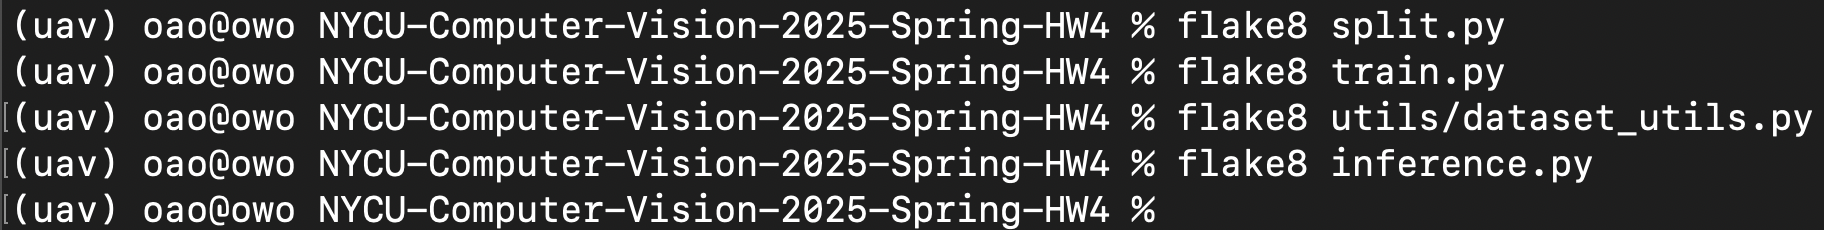
\includegraphics[width=.9\linewidth]{lint_code.png}
\caption{Code quality check (\texttt{flake8}) for reproducibility.}
\end{figure}

\section{References}
\renewcommand{\refname}{}
\begin{thebibliography}{9}
\bibitem{promptir2023}V.~Potlapalli, S.~W.~Zamir, S.~Khan, and F.~S.~Khan, ``PromptIR: Prompting for All-in-One Blind Image Restoration,'' \emph{arXiv preprint arXiv:2306.13090}, 2023.
\end{thebibliography}

\end{document}
